Para el análisis de datos, el paso fundamental es la visualización de estos, dado que sin una imagen clara de la información a trabajar, los especialistas no pueden comparar grupos de datos de forma eficiente. 

"La visualización de datos es la práctica de traducir información en un contexto visual, como un mapa o gráfico, para facilitar que el cerebro humano comprenda y extraiga información útil". \cite{DefinitionDataViz}

De esta manera se facilita la identificación, localización de errores, patrones y cualquier punto a resaltar para su próxima conclusión.

Esta tarea además de importante es compleja, por lo cual necesita de agrupaciones que se encarguen de trabajar en ella constantemente. Estas agrupaciones publican sus esfuerzos en plataformas como GitHub para así poder aportar a la investigación, discutir soluciones, revisar problemas y atraer nuevos colaboradores que permitan el crecimiento y consiguiente eficacia del trabajo.

En esta sección se busca investigar y comparar esos productos probados, refinados y simplificados para dar con el que mejor se adapte a los requerimientos a cubrir. 


% \section{Librerías o frameworks para aplicaciones intensivas de frontend}

%LATE_TODO

\section{Librerías para la visualización de datos}

El gran conjunto de librerías web para la visualización de datos se encuentra dividido en aquellas que dan soporte a uno de los 2 formatos que predominan en el mundo de las visualizaciones web: SVG y Canvas. Ambas tecnologías poseen sus altibajos, por lo que es importante saber identificar cuándo se debe escoger una tecnología sobre otra para resolver el problema planteado. 

El principal problema que posee SVG es su rendimiento a medida que la gráfica crece en complejidad, es decir, aumenta la cantidad de datos. Esto debido a su estructura basada en elementos DOM, los cuales en gran cantidad pueden conducir a un mal rendimiento\cite{SVGPerformance}. Canvas trabaja a un nivel de píxeles (sin almacenar estructuras extra en memoria), por lo que ofrece un mejor rendimiento a medida que los datos aumentan (véase \ref{fig:canvasvssvg}). Por otro lado, el uso de elementos DOM en SVG proporciona una forma fácil de crear gráficas interactivas, ya que cada elemento DOM provee una interfaz para adjuntar eventos Javascript.

Para la selección de librería se consideran los siguientes factores:

\begin{enumerate}
    \item {Debe ser un proyecto open source.}
    \item {De ser posible, debe tener \textit{bindings} \footnote{\textit{Binding}: facilita el uso en ReactJs de una librería hecha en JavaScript vanilla.} de ReactJs para facilidad en el desarrollo.}
    \item {Debe ser extensible para poder implementar aquellas visualizaciones que sean muy específicas.}
    \item {Deben ser longevas y tener cierta garantía de que será mantenida en el tiempo,
    asegurando así que para futuras mejoras de este TEG sigan disponibles.}
    \item {Debe ser fácil de utilizar.}
\end{enumerate}

\begin{figure}[H]
    \centering
    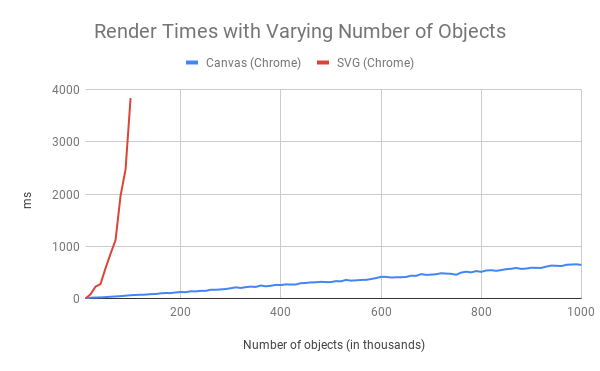
\includegraphics[width=\textwidth]{seminario/images/svg-vs-canvas.png}
    \caption{Comparación de rendimiento entre SVG y Canvas a medida que se incrementa el número de objetos\cite{WhenToUseHTMLCanvas}}
    \label{fig:canvasvssvg}
\end{figure}

A continuación se mostrará el conjunto de librerías de visualización de datos que se escogieron para su comparación. Debido al gran espectro de librerías que existen, solo se mostrarán aquellas que posean la mayor relevancia de acuerdo a los parámetros de búsqueda mencionados anteriormente, usando principalmente GitHub como medio de búsqueda.

\subsection{ Data Driven Documents (D3) }
\begin{itemize}
    \item URL de repositorio: \href{https://github.com/d3/d3}{https://github.com/d3/d3}.
    \item Mantenida por la organización homónima, d3.
\end{itemize}

D3 es una librería Javascript basada en SVG publicada en 2011, que permite manipular documentos basados en datos. D3 permite vincular datos a documentos DOM que después mediante transformaciones del documento sobre los datos se puede construir tablas o gráficas, esto le otorga mucha versatilidad al momento de crear gráficas muy personalizadas e interactivas, pero también agrega una capa de complejidad, ya que las gráficas son construidas \say{a mano}. Además en el ámbito del proyecto (el cual será creado usando ReactJs), D3 no ofrece ningún \textit{binding} para ReactJs por defecto, así que es necesario contemplar el uso de librerías como React-D3-Library\cite{ReactD3Library} que permitan una comunicación sencilla entre ambas tecnologías. 

\subsection{ ECharts }
\begin{itemize}
    \item URL de repositorio: \href{https://github.com/apache/echarts}{https://github.com/apache/echarts}.
    \item Mantenida por Apache.
\end{itemize}

ECharts es una librería Javascript de código abierto creada por Apache que dispone de una gran variedad de tipos de gráficos y la posibilidad de renderizar los gráficos en forma de Canvas, SVG y VML. Además también provee componentes interactivos \say{listos para usarse} que pueden ser agregados a las gráficas para crear leyendas, \textit{tooltips} \footnote{\textit{Tooltip}: elemento gráfico de las interfaces de usuario el cual al hacerle \textit{hover}, muestra información sobre ese elemento.} , enfocar los datos, entre otras cosas.

\section{ Comparación de librerías }

Después de comparar estas librerías, sus APIs y leer otras investigaciones la decisión final es utilizar ECharts.

La base de esta conclusión es la simplicidad \cite{EchartsDecision}, mientras que d3 permite una gran flexibilidad, la curva de aprendizaje tiene una inclinación pronunciada. 
En comparación, ECharts se ve como una herramienta \textit{plug and play} que requiere mínima configuración y ahorra al desarrollador días de esfuerzo.

El tipo de gráficas a utilizar son las siguientes:
\begin{itemize}    
    \item Número.
    \item Línea.
    \item Barra.
    \item Área.
    \item Torta.
    \item Dispersión.
    \item History flow.
\end{itemize}

Para estas gráficas ECharts provee soluciones pre-hechas y si es el caso de gráficos de interés en nichos específicos, como es el caso del History Flow, permite crear gráficas completamente nuevas.
También provee gráficos de Sankey y Stacked Area Chart que son bastante parecidos y podrían ser personalizados para parecerse al History Flow.

\section{ Proyectos alternos }
Estos dos gigantes en el mundo de la visualización de datos por si solos son opciones excelentes, pero trabajan sobre JavaScript vainilla y no están adaptadas para trabajar directamente sobre tecnologías como ReactJS. 
Para facilidad del desarrollo de la aplicación se utilizará una librería que se encargue de adaptar ECharts a ReactJS.

\subsection{ Echarts for React }
\begin{itemize}
    \item URL del repositorio \href{https://github.com/hustcc/echarts-for-react}{https://github.com/hustcc/echarts-for-react}
\end{itemize}

\emph{Echarts for React} es un wrapper que permite usar Echarts en conjunto con ReactJS, de forma que se pueda aprovechar los beneficios que provee el framework. Su uso resulta bastante intuitivo ya que consiste en pasar los parámetros para construir la gráfica a un único componente React \emph{ReactECharts} como se muestra a continuación:

\begin{lstlisting}
    import ReactECharts from 'echarts-for-react';
    const option={...}
    <ReactECharts option={option} /> 
\end{lstlisting}

Donde el parámetro \emph{option} (cuyo contenido fue omitido por simplicidad) provee todas las especificaciones necesarias para crear la gráfica

Además \emph{Echarts for React} ofrece la posibilidad de hacer uso del core de Echarts y de todas las propiedades que este ofrece, tal como la creación de temas, estilos personalizados, \textit{lazy update} \footnote{\textit{Lazy update}: en el contexto de Echarts, \emph{Lazy update} permite actualizar las gráficas de forma asíncrona, ofreciendo mayor control al usuario y gráficas mas optimizadas}





